\documentclass[10pt]{standalone}
\usepackage{mathpazo}\usepackage[T1]{fontenc}\usepackage[utf8]{inputenc}
\usepackage{amsmath,amssymb}
\usepackage{tikz}
\usepackage{xcolor}
\usetikzlibrary{arrows.meta,positioning,fit,backgrounds}

\definecolor{ink}{HTML}{1A1A1A}
\definecolor{acc}{HTML}{1E5B4F}
\definecolor{gry}{HTML}{6B7671}
\definecolor{lgt}{HTML}{C9D2CE}
\definecolor{boxf}{HTML}{F6F8F7}

\newcommand{\hd}{\sffamily\small\bfseries\color{ink}}
\newcommand{\sbb}{\sffamily\scriptsize\color{gry}}
\newcommand{\fm}{\scriptsize\color{ink}}

\begin{document}
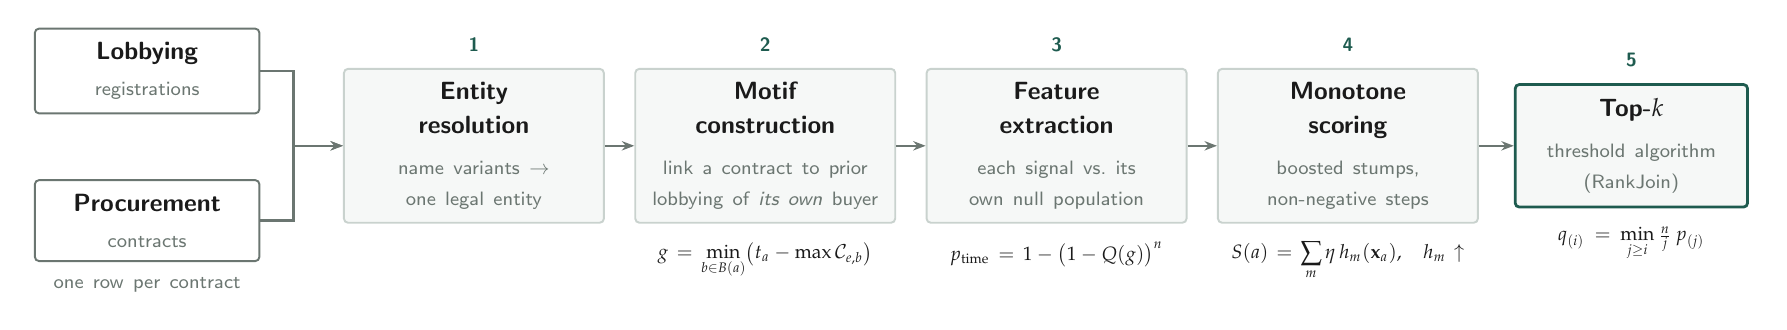
\begin{tikzpicture}[
  font=\sffamily,
  stage/.style ={draw=lgt, fill=boxf, line width=0.7pt, rounded corners=1.5pt,
                 text width=2.95cm, align=center, inner sep=5pt,
                 minimum height=1.55cm},
  src/.style   ={draw=gry, line width=0.7pt, rounded corners=1.5pt,
                 text width=2.5cm, align=center, inner sep=5pt,
                 minimum height=0.95cm},
  outb/.style   ={draw=acc, fill=boxf, line width=1.0pt, rounded corners=1.5pt,
                 text width=2.6cm, align=center, inner sep=5pt,
                 minimum height=1.55cm},
  a/.style     ={-{Stealth[length=4.5pt]}, draw=gry, line width=0.8pt},
  num/.style   ={font=\sffamily\scriptsize\bfseries, color=acc}
]

% ---------------- sources
\node[src] (l) at (0, 0.95)  {{\hd Lobbying}\\[1pt]{\sbb registrations}};
\node[src] (p) at (0,-0.95)  {{\hd Procurement}\\[1pt]{\sbb contracts}};

% ---------------- stages
\node[stage] (er) at (4.15,0)
  {{\hd Entity\\resolution}\\[3pt]{\sbb name variants $\rightarrow$}\\[-1pt]{\sbb one legal entity}};

\node[stage] (mc) at (7.85,0)
  {{\hd Motif\\construction}\\[3pt]{\sbb link a contract to prior}\\[-1pt]{\sbb lobbying of \emph{its own} buyer}};

\node[stage] (fe) at (11.55,0)
  {{\hd Feature\\extraction}\\[3pt]{\sbb each signal vs.\ its}\\[-1pt]{\sbb own null population}};

\node[stage] (sc) at (15.25,0)
  {{\hd Monotone\\scoring}\\[3pt]{\sbb boosted stumps,}\\[-1pt]{\sbb non-negative steps}};

\node[outb] (tk) at (18.85,0)
  {{\hd Top-$k$}\\[3pt]{\sbb threshold algorithm}\\[-1pt]{\sbb (RankJoin)}};

% ---------------- flow
\draw[a] (l.east) -- ++(0.42,0) |- (er.west);
\draw[a] (p.east) -- ++(0.42,0) |- (er.west);
\draw[a] (er) -- (mc);
\draw[a] (mc) -- (fe);
\draw[a] (fe) -- (sc);
\draw[a] (sc) -- (tk);

% ---------------- numbering
\node[num, above=2.5pt of er] {1};
\node[num, above=2.5pt of mc] {2};
\node[num, above=2.5pt of fe] {3};
\node[num, above=2.5pt of sc] {4};
\node[num, above=2.5pt of tk] {5};

% ---------------- formulas beneath
\node[below=3pt of mc, text width=3.5cm, align=center]
  {\fm $g=\displaystyle\min_{b\in B(a)}\bigl(t_a-\max\mathcal{C}_{e,b}\bigr)$};

\node[below=3pt of fe, text width=3.5cm, align=center]
  {\fm $p_{\mathrm{time}}=1-\bigl(1-Q(g)\bigr)^{n}$};

\node[below=3pt of sc, text width=3.6cm, align=center]
  {\fm $S(a)=\displaystyle\sum_{m} \eta\,h_m(\mathbf{x}_a),\ \ h_m\uparrow$};

\node[below=3pt of tk, text width=3.0cm, align=center]
  {\fm $q_{(i)}=\displaystyle\min_{j\ge i}\tfrac{n}{j}\,p_{(j)}$};

% ---------------- one-line captions under sources
\node[below=2pt of p, text width=2.8cm, align=center]
  {\sbb one row per contract};

\end{tikzpicture}
\end{document}
